\subsection{Affinity Propagation}

Affinity Propagation is a clustering algorithm that identifies a set of \textit{exemplars} that represents the dataset\footnote{Brendan J. Frey, Delbert Dueck, \emph{Clustering by Passing Messages
Between Data Points}, http://www.sciencemag.org/, 2007}. The input of Affinity Propagation is the pair-wise similarities between each pair of data points, $s[i, j] \forall i, j = 1, \ldots, n$\footnote{$s[i,j]$ for each data point is called preference and impacts the number of clusters.}. Any type of similarities is acceptable thus Affinity Propagation is widely applicable.

Given similarity matrix $s[i, j]$, Affinity Propagation attempts to find the exemplars that maximize the net similarity, i.e. the overall sum of similarities between all exemplars and their member data points. The process of Affinity Propagation can be viewed as a message passing process with two
kinds of messages exchanged among data points: \emph{responsibility} and \emph{availability}. 

Responsibility, $r[i, j]$, is a message from data point $i$ to $j$ that reflects the accumulated evidence for how well-suited data point j is to serve as the exemplar for data point i. 

Availability, $a[i, j]$, is a message from data point $j$ to $i$ that reflects the accumulated evidence for how appropriate it would be for data point $i$ to choose data point $j$ as
its exemplar. All responsibilities and availabilities are set to $0$ initially, and their values are iteratively updated as follows to compute convergence values:

$$r[i, j] = (1-\lambda)\rho [i, j] + \lambda r[i, j]$$
$$a[i, j] = (1 -\lambda) \alpha[i, j] + \lambda a[i, j]$$

where $\lambda$ is a damping factor introduced to avoid numerical oscillations, and $\rho[i, j]$ and $\alpha[i, j]$ are, we call, \emph{propagating responsibility} and \emph{propagating availability}, respectively. 

$\rho[i, j]$ and $\alpha[i, j]$ are computed by the following equations:

$$
\rho[i, j] =
\left\{
\begin{array}{lr}
s[i, j] − \max_{k=j}a[i, k] + s[i, k] & i \neq j\\
s[i, j] − \max_{k=j}s[i, k]  &  i= j 
\end{array}
\right.
$$
$$
\alpha[i, j] =
\left\{
\begin{array}{lr}
min{0, r[j, j] + \sum_{k \neq i, j} \max 0, r[k, j]} & i \neq j\\
\sum_{k\neq j} \max {0, r[k, j]}  &  i= j 
\end{array}
\right.
$$

That is, messages between data points are computed from the corresponding propagating messages. The exemplar of data point $i$ is finally defined as:

$$arg \max {r[i, j] + a[i, j] : \forall \; j = 1, 2, \ldots,n}$$

As described above, the original algorithm requires $O(n^2 t)$ time to update massages, where $n$ and $t$ are the number of data points and the number of iterations, respectively.
This incurs excessive CPU time, especially when the number of data points is large\footnote{Yasuhiro Fujiwara, Go Irie, Tomoe Kitahara, \emph{Fast Algorithm for Affinity Propagation}, 2009}. The Figure \ref{fig:ap} shows how affinity propagation works\footnote{Brendan J. Frey, Delbert Dueck, \emph{op. cit.}, Figure 1, p. 974}.

\begin{figure}[!htbp]
\centering
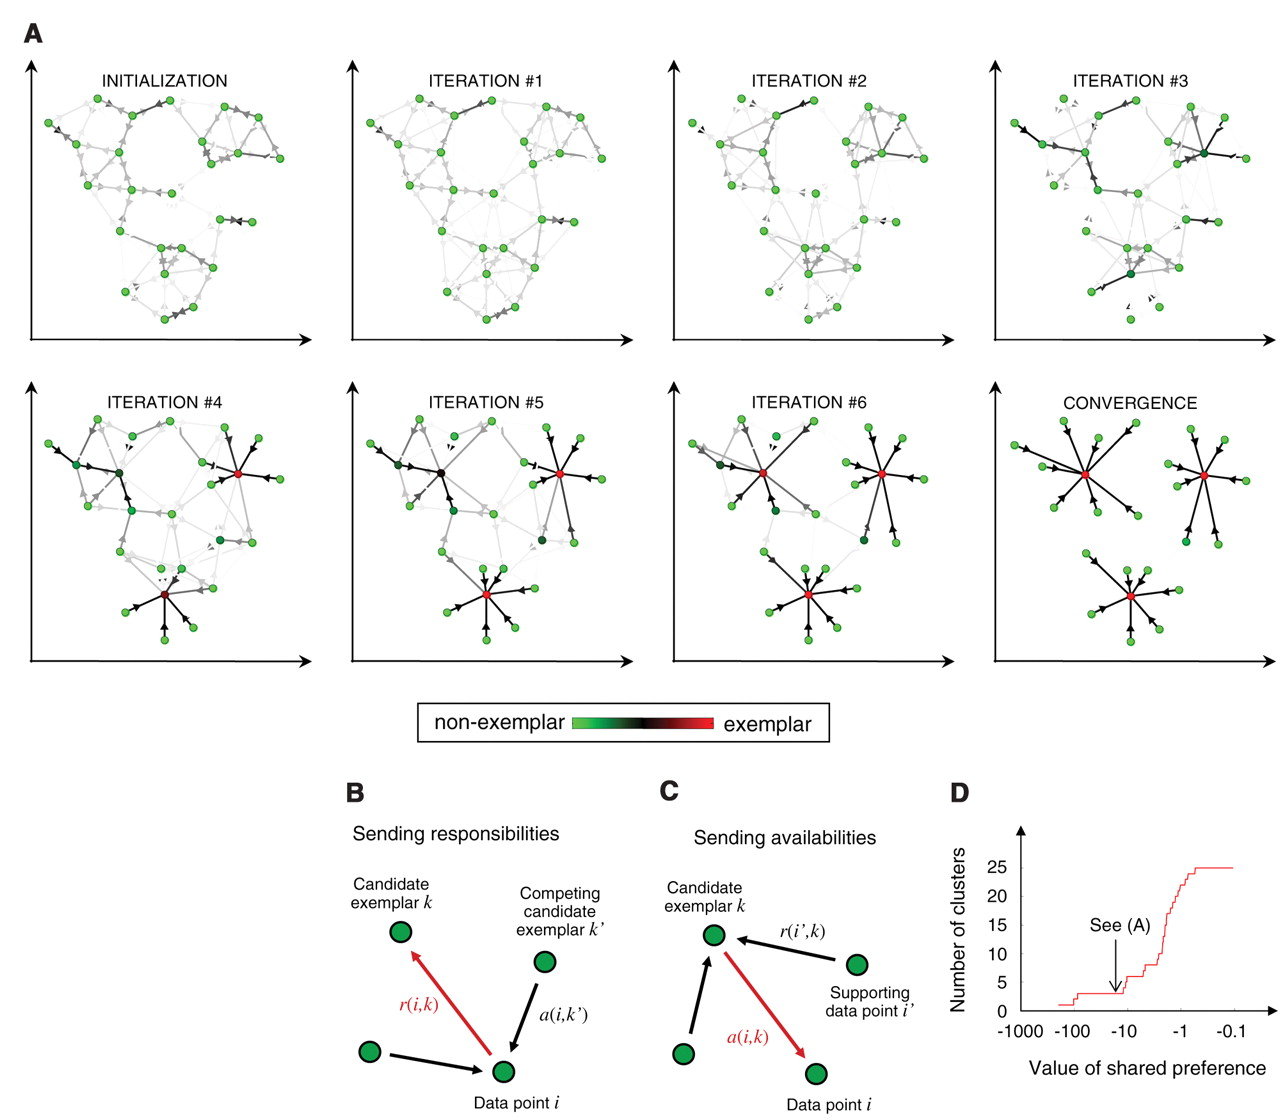
\includegraphics[width=0.73\textwidth]{images/ap.jpg}
\caption{How affinity propagation works}
\label{fig:ap}
\end{figure}

The clustering process described is then applied to the array of similarity calculated previously on features extracted from each words. Once you have run the calculation of clusters, segments are organized into individual folders to provide a visual result of the proceedings just completed. Each group is identified by a segment that represents the centroid of the cluster, which is the element to which all others in the group are closer.